%! TEX root = diss.tex
\documentclass[../diss.tex]{subfiles}

\appendix

\chapter{Further definitions}%
\label{cha:Further definitions}

\section{Abstract algebra}%
\label{sec:Abstract algebra}

TODO

\chapter{Other}

\section{Word count}%
\label{sec:Word count}

The word count was computed by concatenating the 5 chapters and using {\TeX}count.
I used the following script to do this:
\begin{verbatim}
echo "$(head -n 4 diss.tex)
    $(tail -n +3 -q sections/*.tex)
    $(tail diss.tex -n +5 -q)" | \
    texcount - $@ -sub=chapter | \
    grep -P "Introduction|Preparation|Implementation|Evaluation|Conclusions" | \
    grep -oP "\d+[+]\d+[+]\d+" | \
    bc | \
    awk '{s+=$1} END {print s}'
\end{verbatim}

% Error bars {{{
\section{Error bars}%
\label{sec:Error bars}

The plots with error bars:

% Sandy bridge
\begin{figure}
    \begin{center}
        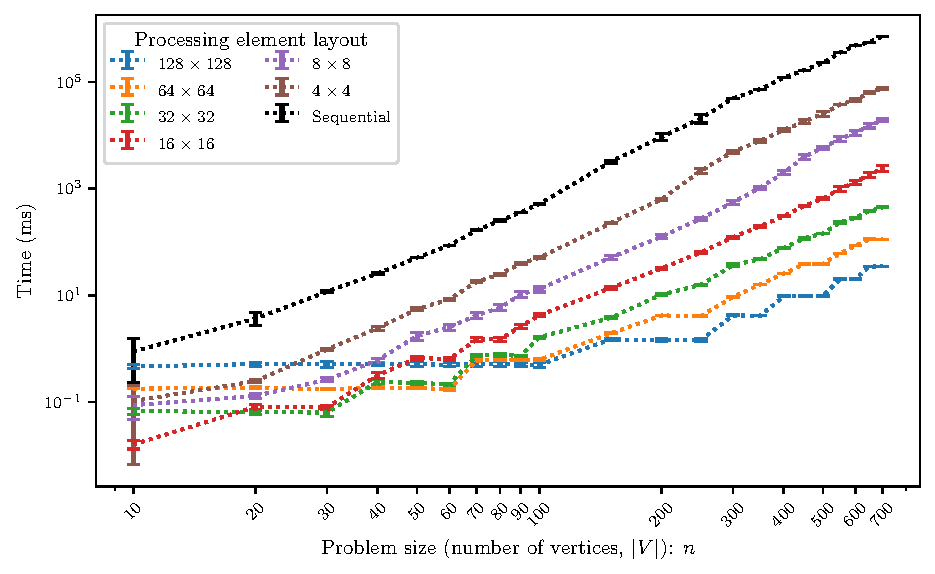
\includegraphics{figs/plots/total-time-scaling-sandy-full-width.pdf}
    \end{center}
    \caption{Sandy bridge total time scaling}
    \label{fig:appendix-plot-sandy-bridge}
\end{figure}

% Taihu light
\begin{figure}
    \begin{center}
        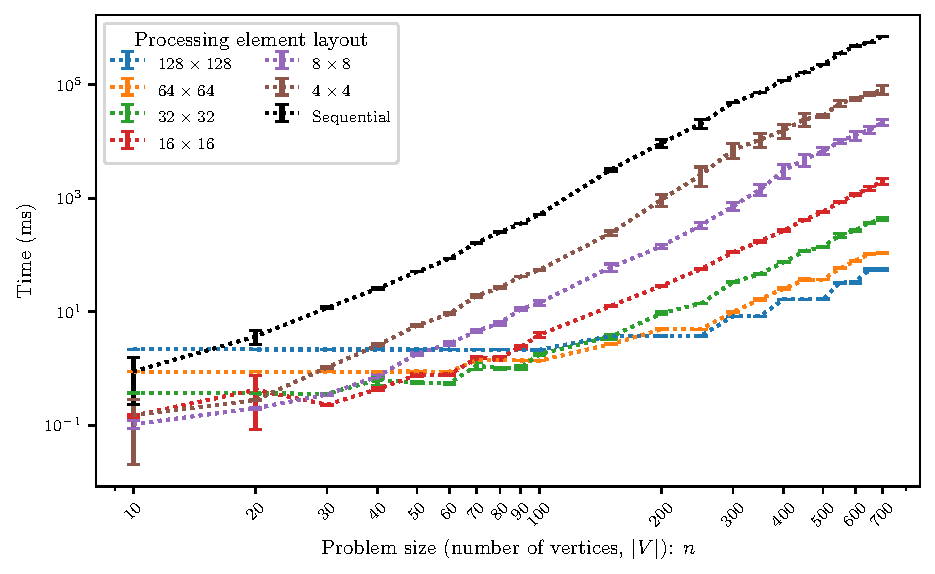
\includegraphics{figs/plots/total-time-scaling-taihu-full-width.pdf}
    \end{center}
    \caption{Taihu-Light total time scaling}
    \label{fig:appendix-plot-taihu-light}
\end{figure}

% Internet
\begin{figure}
    \begin{center}
        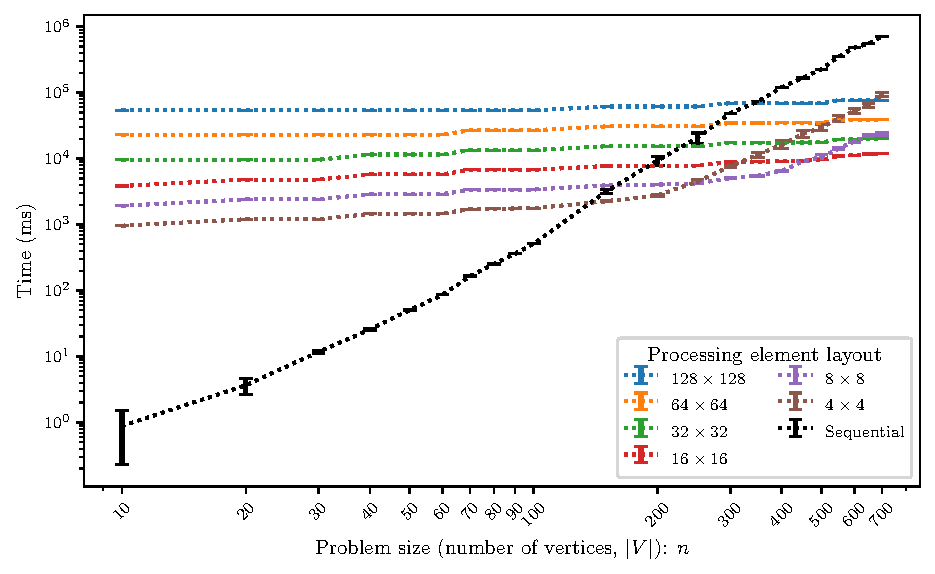
\includegraphics{figs/plots/total-time-scaling-internet-full-width.pdf}
    \end{center}
    \caption{Internet total time scaling}
    \label{fig:appendix-plot-internet}
\end{figure}

% }}}

\section{Path reconstruction}%
\label{sec:path-reconstruction}

As an example of the path reconstruction algorithm presented in
\cref{sec:APSP via repeated matrix-squaring}, consider the completed predecessor
matrix for the graph in
\cref{fig:example-graph}:
\begin{equation}
    M_{pred}=
    \begin{blockarray}{ccccccccc}
         & 0 & 1 & 2 & 3 & 4 & 5 & 6 & 7 \\
        \begin{block}{c(cccccccc)}
            0 & 0 & 5 & 0 & 0 & 1 & 2 & 2 & 7 \\
            1 & 0 & 1 & 2 & 3 & 1 & 5 & 6 & 7 \\
            2 & 0 & 5 & 2 & 3 & 1 & 2 & 2 & 7 \\
            3 & 0 & 1 & 2 & 3 & 4 & 5 & 3 & 7 \\
            4 & 0 & 1 & 2 & 3 & 4 & 5 & 6 & 7 \\
            5 & 0 & 5 & 2 & 3 & 1 & 5 & 6 & 7 \\
            6 & 0 & 1 & 2 & 3 & 4 & 5 & 6 & 7 \\
            7 & 0 & 1 & 2 & 3 & 4 & 5 & 6 & 7 \\
        \end{block}
    \end{blockarray}\;.
\end{equation}
If we want to reconstruct $0 \rightsquigarrow 1$, we start with
the list $[1]$, then prepend $M_{pred}[0,1]=5$, giving $[5,1]$. We then prepend
$M_{pred}[0,5]=2$. We continue doing this until we get $[0,2,5,1]$, where we
stop because $M_{pred}[0,0]=0$.


% Project proposal
\chapter{Project Proposal}

\newlength{\originalVOffset}
\newlength{\originalHOffset}
\setlength{\originalVOffset}{\voffset}   
\setlength{\originalHOffset}{\hoffset}

\setlength{\voffset}{0cm}
\setlength{\hoffset}{0cm}
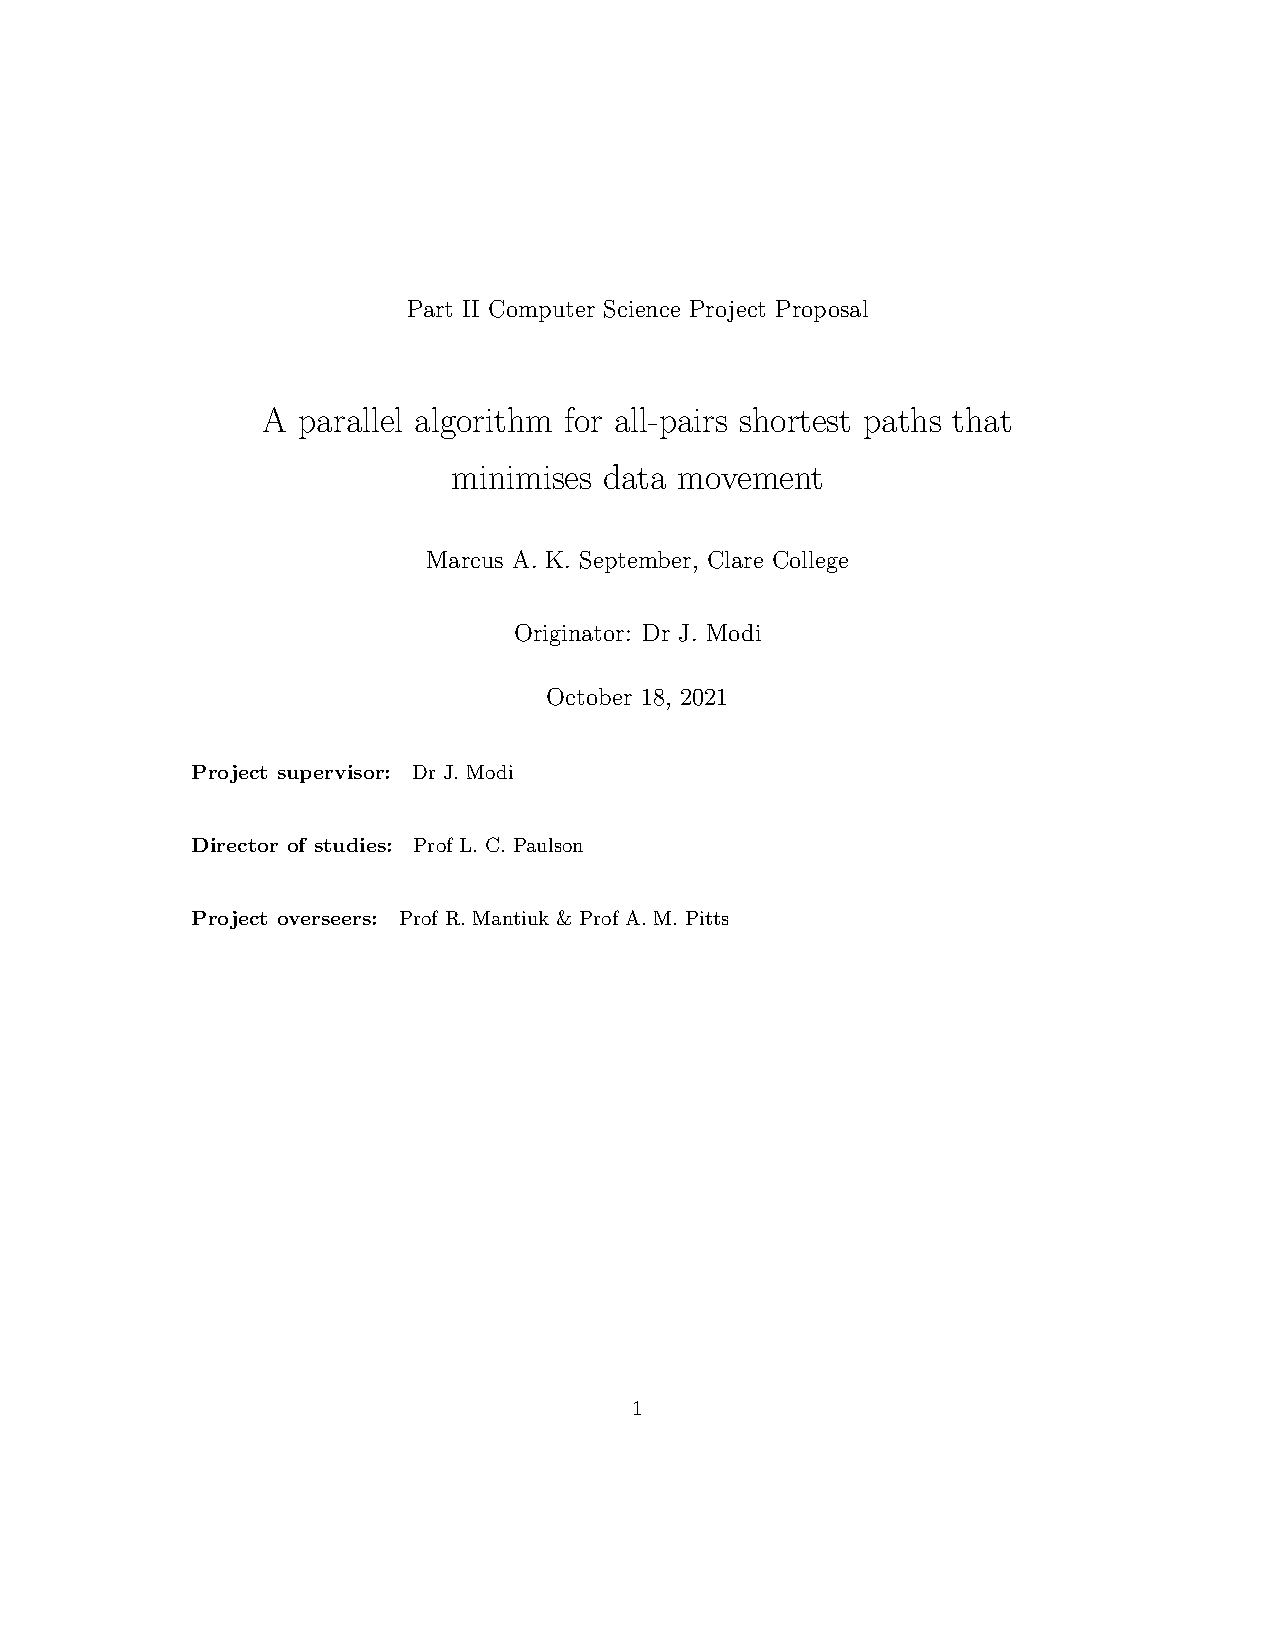
\includepdf[pages=-]{../project-proposal/proposal} \setlength{\voffset}{\originalVOffset}
\setlength{\hoffset}{\originalHOffset}
% \subfile{../project-proposal/proposal}
